\begin{frame}[c]
 \frametitle{RSTC Network}
 \framesubtitle{multi-layer receptor-signaling-transcription-cell state}
%\begin{beamer}

\begin{center}
  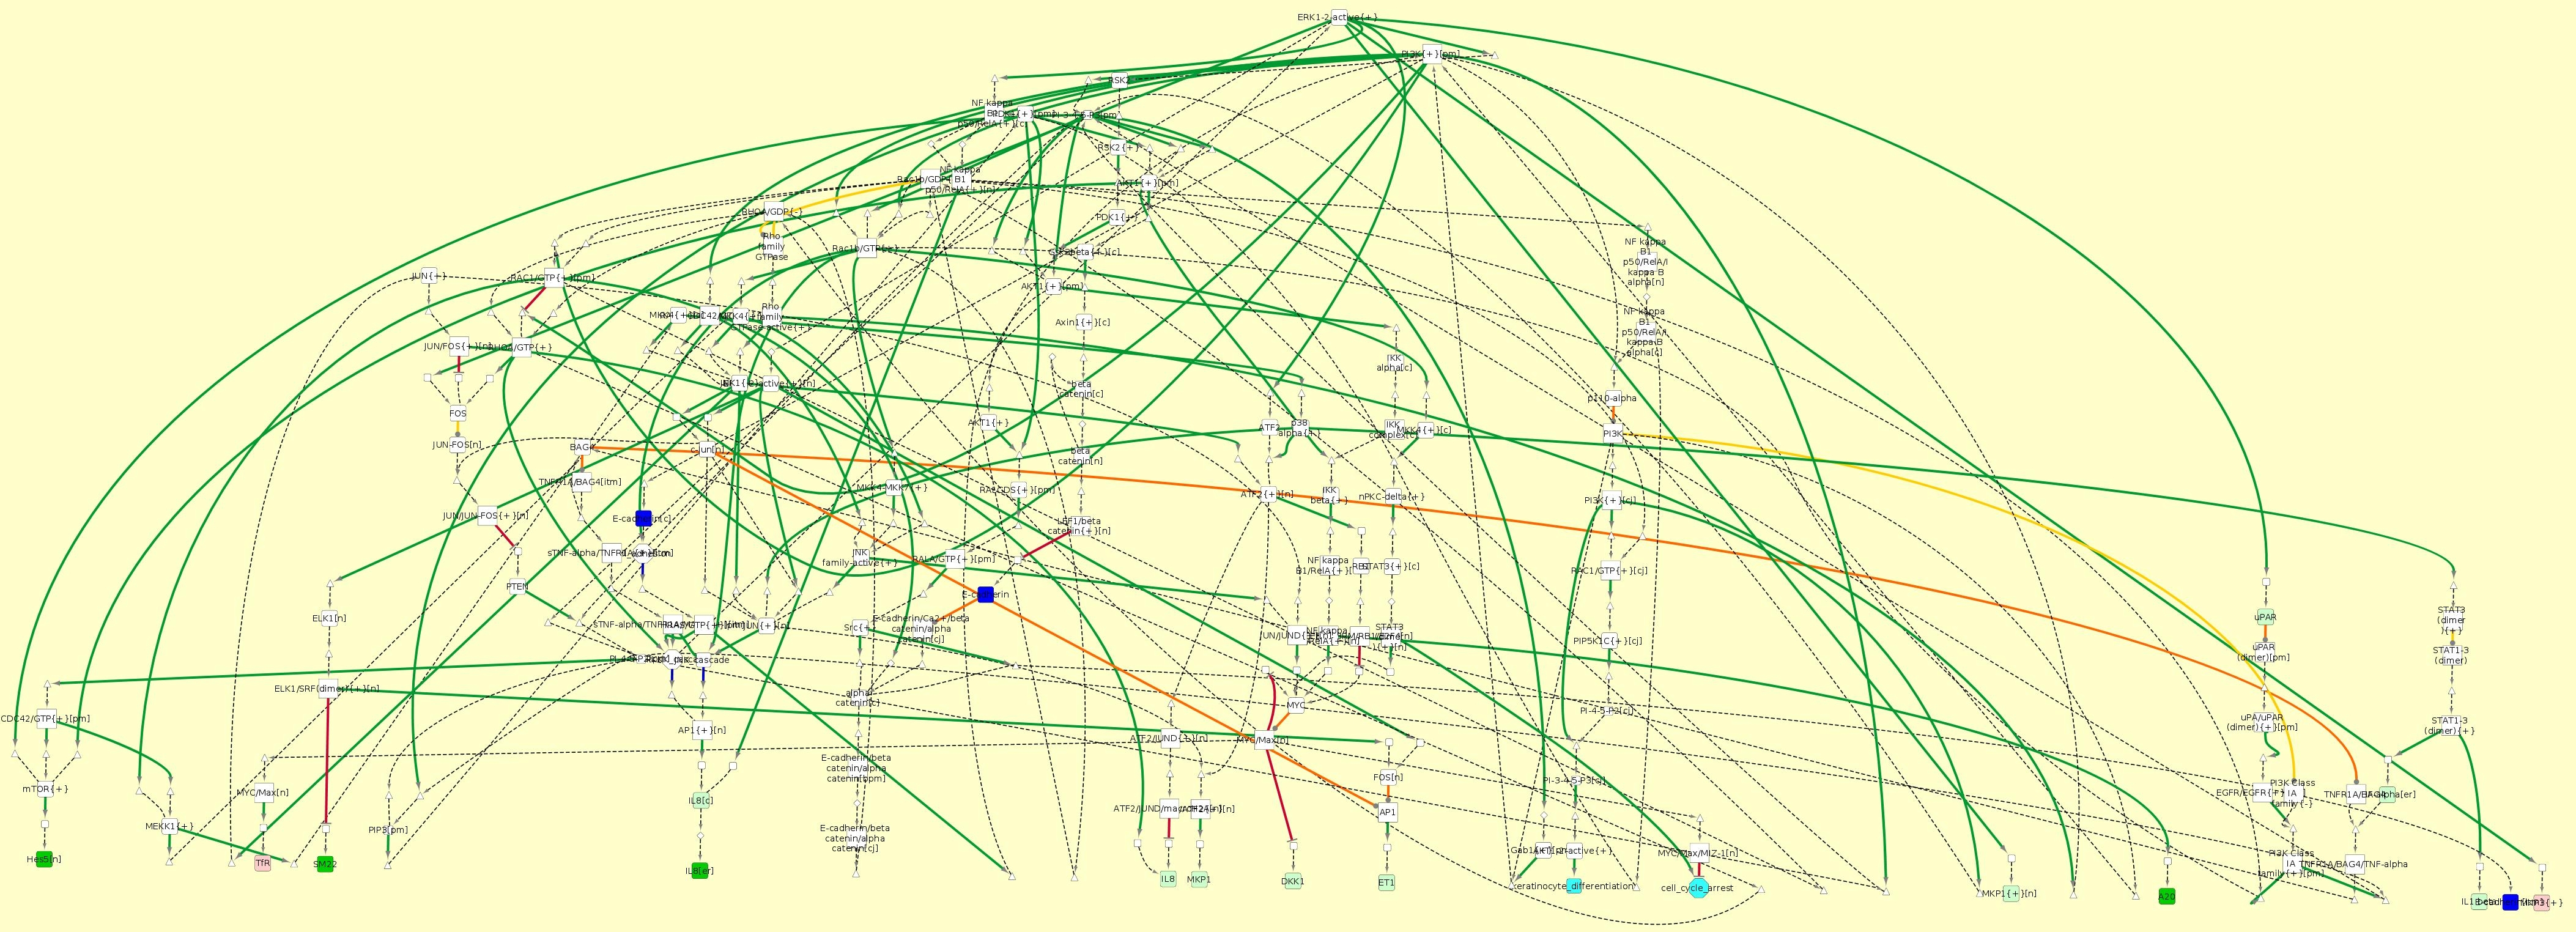
\includegraphics[scale=0.07]{figs/net.jpg}
\end{center}
 
%\end{beamer}

%\pause

\begin{itemize}
 \item Pathway Interaction Database
 \item \tval{$293$  nodes}: signaling proteins, transcription factors, mRNA expressions
 \item \tval{$375$  interactions}: activations, inhibitions, complexes dissociation
\end{itemize}

 
\end{frame}

\begin{frame}[c]
 \frametitle{RSTC Network}
 \framesubtitle{multi-layer receptor-signaling-transcription-cell state}

%%%image zoomée
\begin{tikzpicture}[node distance = 1em,dashed,red,thick]
	\zoomZero{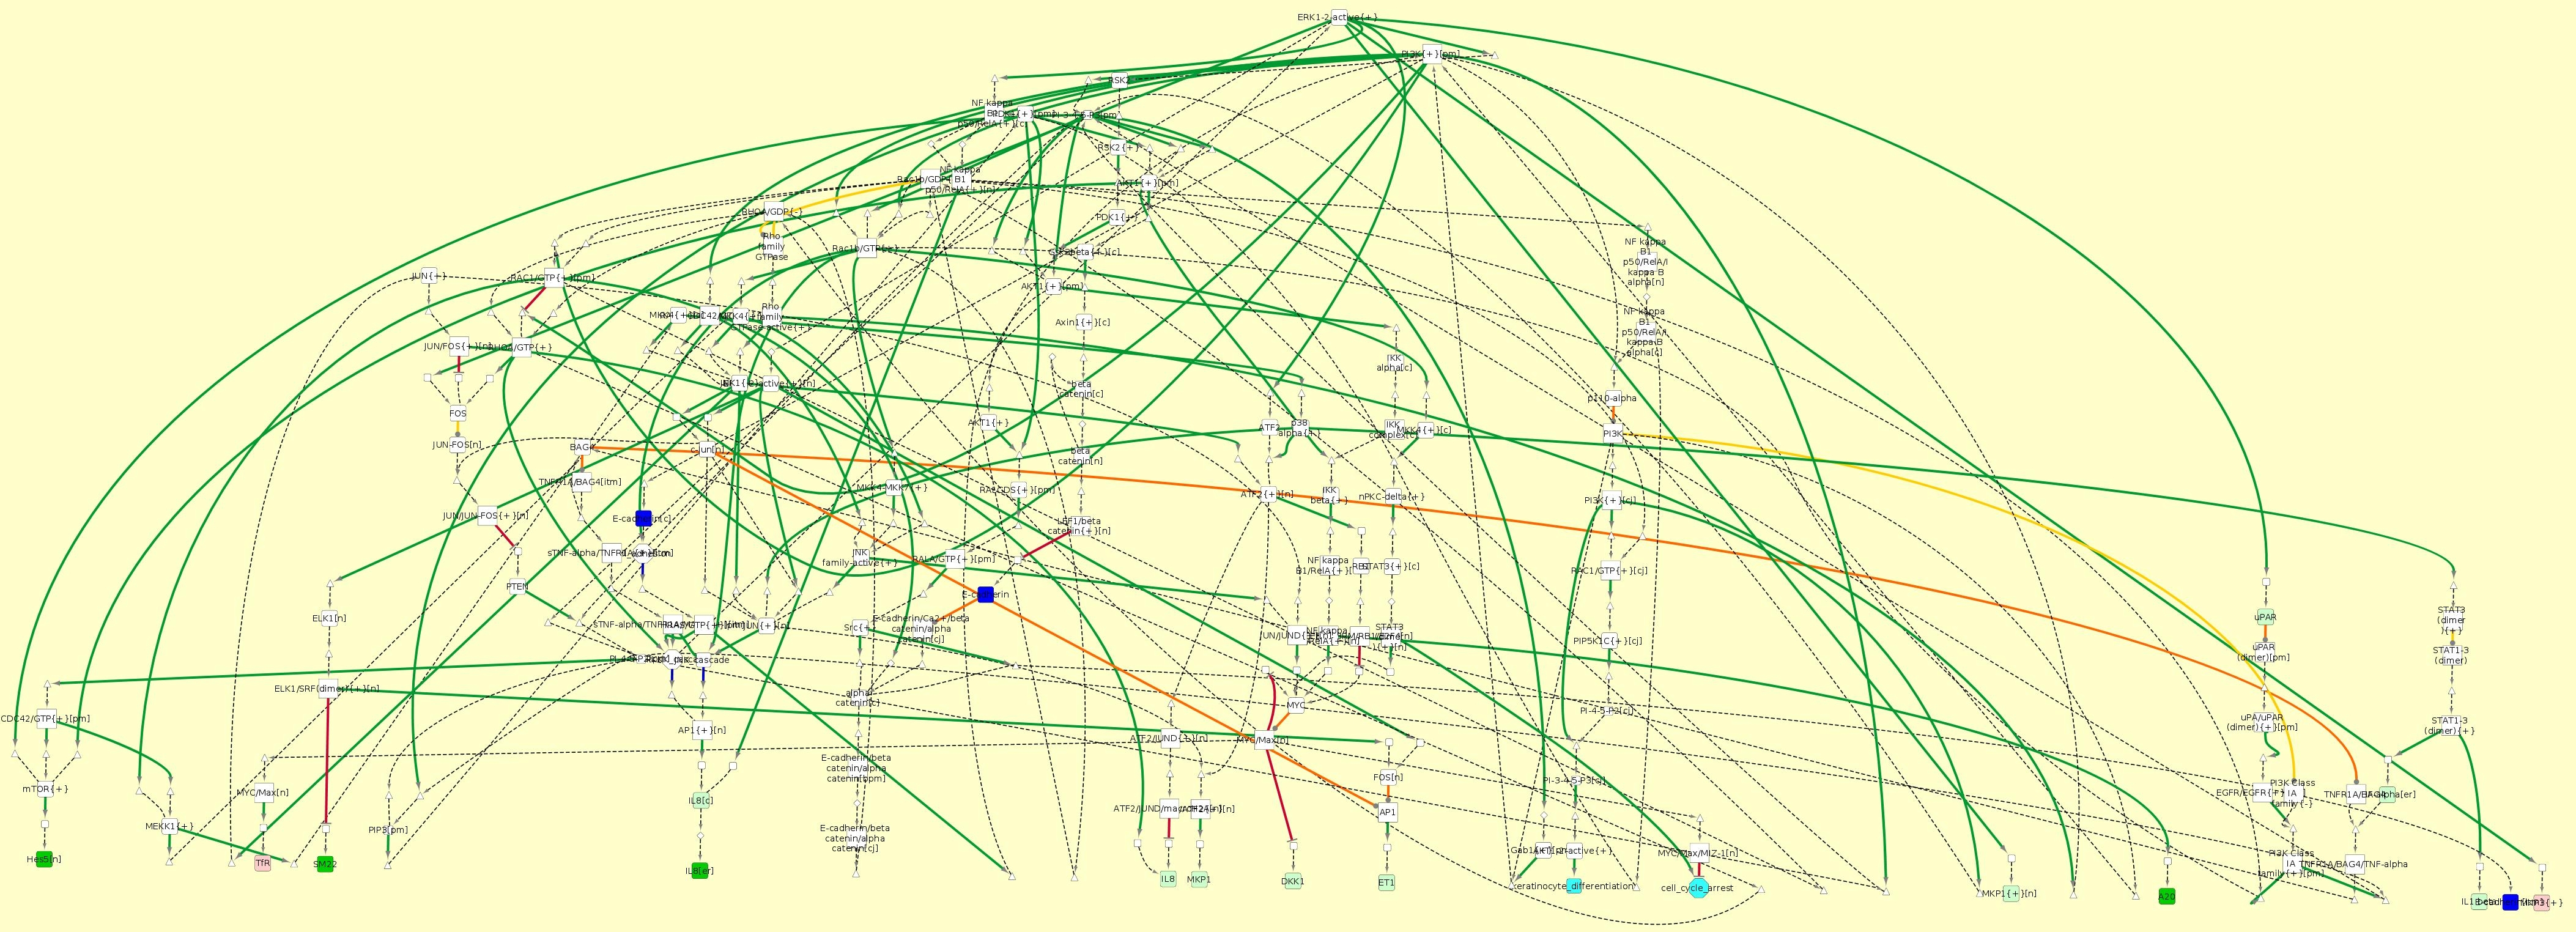
\includegraphics[width=0.35\textwidth]{figs/net.jpg}}
	\zoomIn[right]{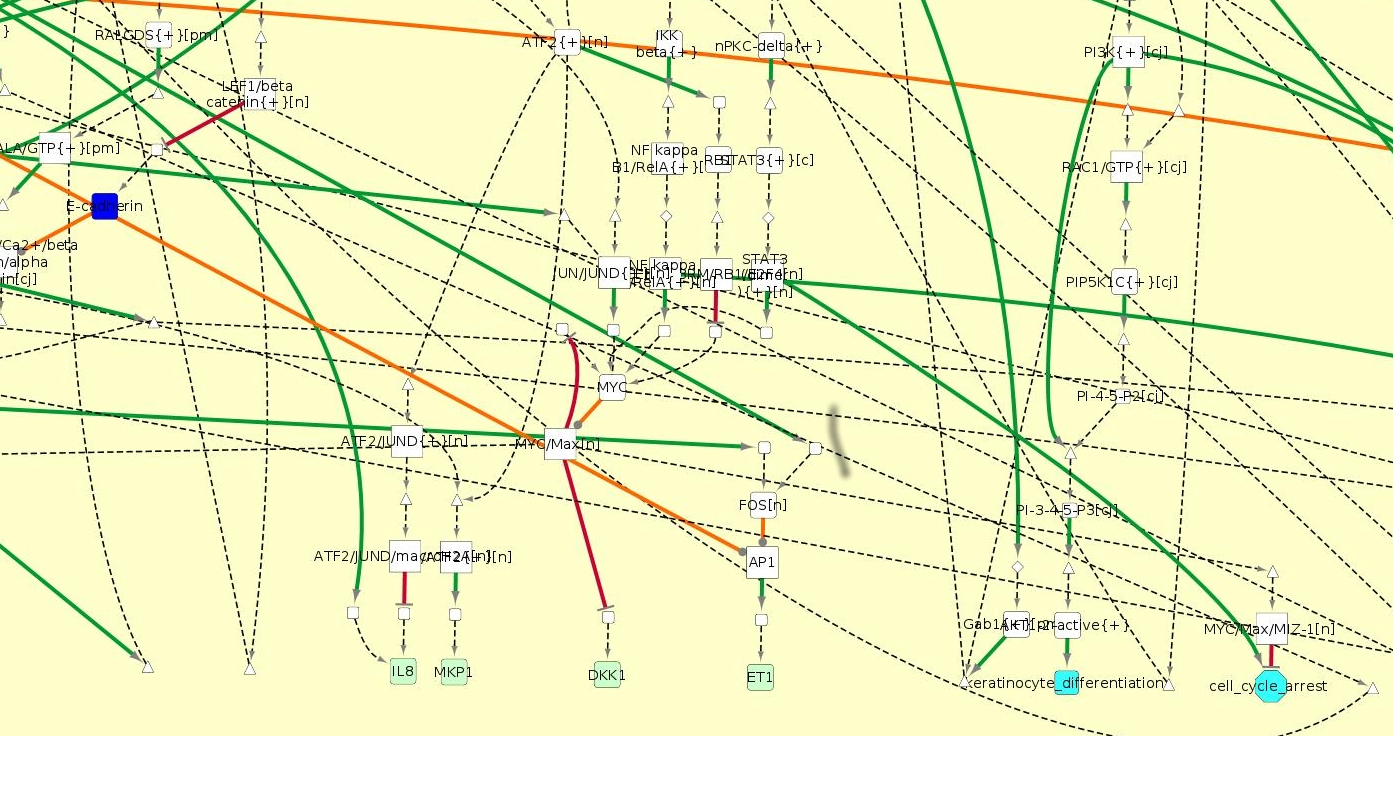
\includegraphics[scale=0.15]{figs/netzoom.png}}{0.35,0.005}{0.320,0.420}
	%\zoomIn{\includegraphics[width=0.45\textwidth]{Geant3}}{0.45,0.475}{0.120,0.120}
	%\zoomIn[left]{\includegraphics[width=0.45\textwidth]{Geant2}}{0.45,0.475}{0.120,0.120}
	%\zoomIn{\includegraphics[width=0.45\textwidth]{Geant1}}{0.45,0.475}{0.120,0.120}
	%\zoomIn[right]{\includegraphics[width=0.45\textwidth]{Geant0}}{0.45,0.475}{0.120,0.120}
\end{tikzpicture}


\end{frame}

\begin{frame}[c]
 \frametitle{RSTC Network}
 \framesubtitle{multi-layer receptor-signaling-transcription-cell state}

%%%image zoomée
\begin{tikzpicture}[node distance = 1em,dashed,red,thick]
	\zoomZero{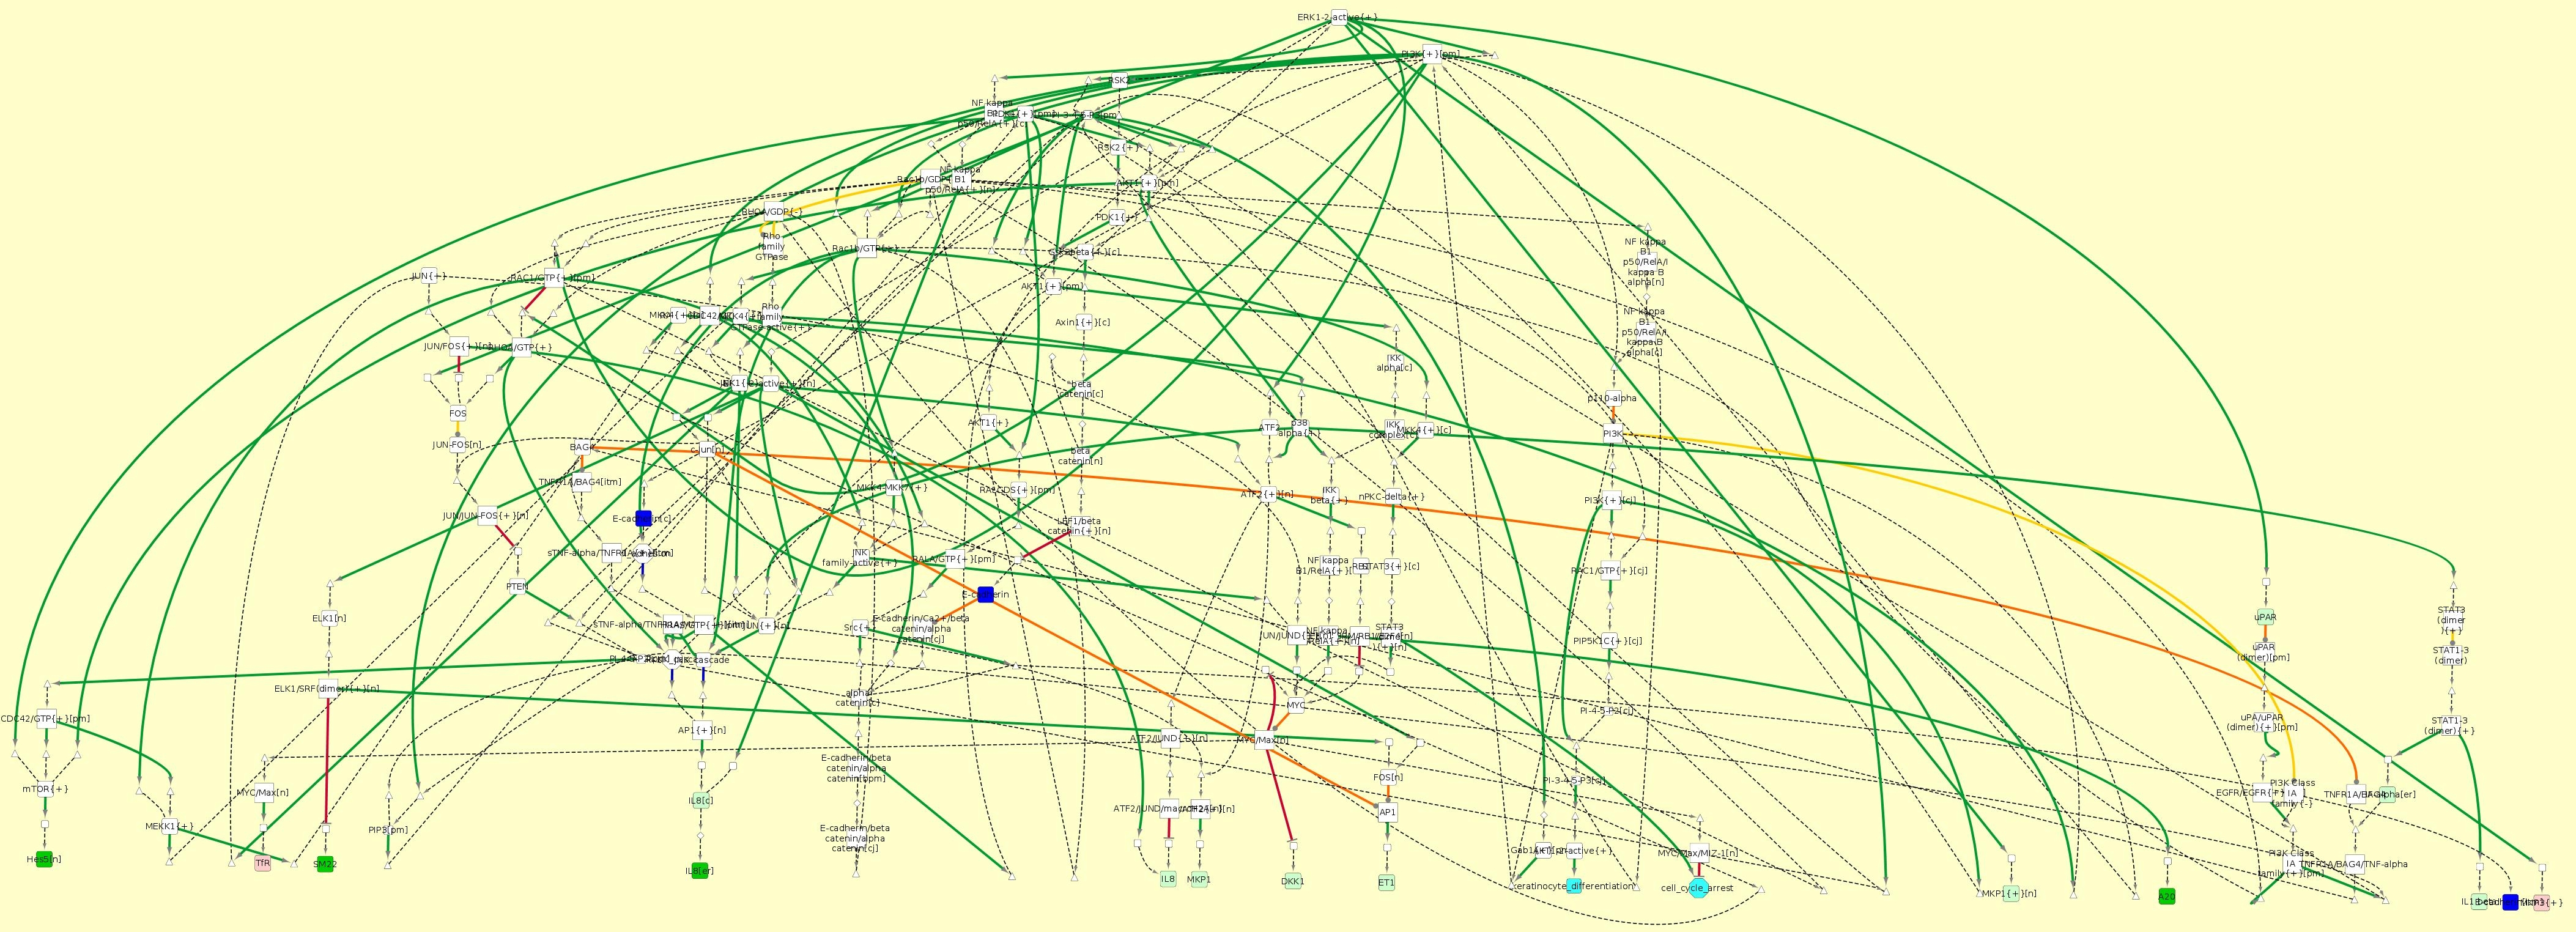
\includegraphics[width=0.45\textwidth]{figs/net.jpg}}
	\zoomIn[left]{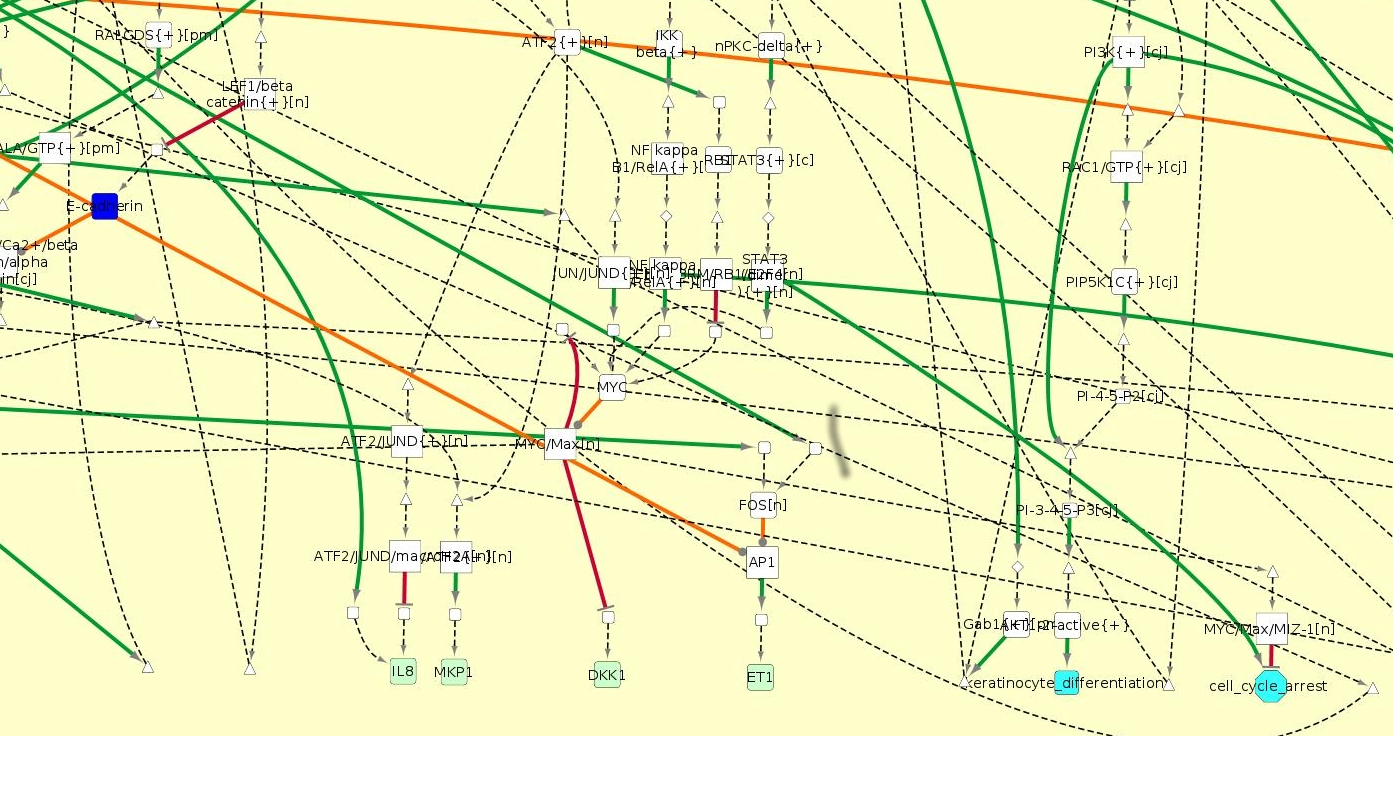
\includegraphics[scale=0.25]{figs/netzoom.png}}{0.35,0.005}{0.320,0.420}
	%\zoomIn{\includegraphics[width=0.45\textwidth]{Geant3}}{0.45,0.475}{0.120,0.120}
	%\zoomIn[left]{\includegraphics[width=0.45\textwidth]{Geant2}}{0.45,0.475}{0.120,0.120}
	%\zoomIn{\includegraphics[width=0.45\textwidth]{Geant1}}{0.45,0.475}{0.120,0.120}
	%\zoomIn[right]{\includegraphics[width=0.45\textwidth]{Geant0}}{0.45,0.475}{0.120,0.120}
\end{tikzpicture}


\end{frame}
